This appendix presents additional regression tables of the paper. 
% RAW ESTIMATE
Table \ref{chap3-tab:reg-v5-raw-all-long} presents the long-version table of the regression table \ref{chap3-tab:reg-v5-raw-all-short} in the paper.
% INSTRUMENTAL VARIABLE
Table \ref{chap3-tab:reg-v5-IV-GFGC-long} presents the IV estimate of the spillover effects. Tables \ref{chap3-tab:reg-v5-IV-GFvote} and \ref{chap3-tab:reg-v5-IV-GCvote} correspond to the IV estimate of the group membership.
% SEM
Table \ref{chap3-tab:reg-v5-sem-GF-stage12}, \ref{chap3-tab:reg-v5-sem-GC-stage12}, and \ref{chap3-tab:reg-v5-sem-BU-stage12} present the details of the 2SLS estimates of the SEM for, respectively, the girl-first, got-cancer, and been-unemployed life event.
% DECOMPOSITION
Tables \ref{chap3-tab:decomp-GF}, \ref{chap3-tab:decomp-GC}, and \ref{chap3-tab:decomp-BU} summarize the decomposition of the total effect from the SEM for, respectively, the girl-first, got-cancer, and been-unemployed life event.
% ROBUSTNESS
Figure \ref{chap3-fig:sem-decomp-v5-GFGender} summarizes the decomposition of the total
effect of girl-first life event by parent. 
Figure \ref{chap3-fig:sem-decomp-v5-GFEduc} summarizes the decomposition of the total
effect of girl-first life event by education level.
Figure \ref{chap3-fig:sem-decomp-v5-BUActivity} summarizes the decomposition of the total
effect of been-unemployed life event according to the current activity status.

%%%%% APPLIED %%%%%

\begin{table}[!htb]
    \centering
    \caption{Effect of life events on values}
    \label{chap3-tab:reg-v5-raw-all-long}
    % \resizebox*{\textwidth}{!}{
    \begin{threeparttable}
        \setlength{\tabcolsep}{0pt}
        \begin{tabular}{l D{.}{.}{5.5} D{.}{.}{5.5} D{.}{.}{5.5} D{.}{.}{5.5} D{.}{.}{5.5} D{.}{.}{5.5}}
\toprule
 & \multicolumn{6}{c}{Linear regression - OLS} \\
\cmidrule(lr){2-7}
 & \multicolumn{2}{c}{GirlFirst} & \multicolumn{2}{c}{GotCancer} & \multicolumn{2}{c}{BeenUnemp} \\
\cmidrule(lr){2-3}\cmidrule(lr){4-5}\cmidrule(lr){6-7}
 & \multicolumn{1}{c}{(Cons)} & \multicolumn{1}{c}{(Coll)} & \multicolumn{1}{c}{(Cons)} & \multicolumn{1}{c}{(Coll)} & \multicolumn{1}{c}{(Cons)} & \multicolumn{1}{c}{(Coll)} \\
\midrule
Intercept       & 0.32^{***}  & -0.15^{***} & 0.27^{***}  & -0.07^{***} & 0.26^{***}  & -0.11^{***} \\
                & (0.02)      & (0.02)      & (0.01)      & (0.01)      & (0.01)      & (0.01)      \\
Female          & -0.19^{***} & 0.07^{***}  & -0.17^{***} & 0.02        & -0.17^{***} & 0.03^{***}  \\
                & (0.01)      & (0.01)      & (0.01)      & (0.01)      & (0.01)      & (0.01)      \\
Educ. Secondary & -0.29^{***} & -0.04^{**}  & -0.28^{***} & -0.03^{**}  & -0.28^{***} & -0.03^{**}  \\
                & (0.02)      & (0.02)      & (0.01)      & (0.01)      & (0.01)      & (0.01)      \\
Educ. Tertiary  & -0.52^{***} & -0.04^{**}  & -0.50^{***} & -0.03^{**}  & -0.50^{***} & -0.03^{***} \\
                & (0.02)      & (0.02)      & (0.01)      & (0.01)      & (0.01)      & (0.01)      \\
Life event      & 0.03^{**}   & 0.00        & 0.09^{***}  & 0.02        & 0.02^{*}    & 0.18^{***}  \\
                & (0.01)      & (0.01)      & (0.03)      & (0.03)      & (0.01)      & (0.01)      \\
Value$_{t-1}$   & 0.54^{***}  & 0.49^{***}  & 0.56^{***}  & 0.50^{***}  & 0.56^{***}  & 0.49^{***}  \\
                & (0.01)      & (0.01)      & (0.00)      & (0.00)      & (0.00)      & (0.00)      \\
\midrule
R$^2$ & \multicolumn{1}{c}{0.37} & \multicolumn{1}{c}{0.26} & \multicolumn{1}{c}{0.39} & \multicolumn{1}{c}{0.27} & \multicolumn{1}{c}{0.39} & \multicolumn{1}{c}{0.27}\\
Adj. R$^2$ & \multicolumn{1}{c}{0.37} & \multicolumn{1}{c}{0.26} & \multicolumn{1}{c}{0.39} & \multicolumn{1}{c}{0.27} & \multicolumn{1}{c}{0.39} & \multicolumn{1}{c}{0.27}\\
Num. obs. & \multicolumn{1}{c}{23354} & \multicolumn{1}{c}{23354} & \multicolumn{1}{c}{32885} & \multicolumn{1}{c}{32885} & \multicolumn{1}{c}{32885} & \multicolumn{1}{c}{32885}\\
\bottomrule
\end{tabular}

        \begin{tablenotes}[flushleft]
            \footnotesize{\item \textit{Notes}: $^{***}p<0.01$; $^{**}p<0.05$; $^{*}p<0.1$. Standard errors between parentheses. Male in the NCDS cohort in his forties with primary education as the reference group. GirlFirst and GotCancer are the life events. In GirlFirst regressions, parents who have had a boy as a first child are the reference group. In GotCancer regressions, individuals who never had a cancer are the reference group. In BeenUnemp, individuals who have never been unemployed are the reference group. Table \ref{chap3-tab:reg-v5-raw-all-short} in the paper summarizes the coefficients.}
        \end{tablenotes}
    \end{threeparttable}
    % }
\end{table}

\begin{table}[!htb]
    \centering
    \caption{IV Estimate of the spillover effect}
    \label{chap3-tab:reg-v5-IV-GFGC-long}
    \begin{threeparttable}
        \begin{tabular}{l D{.}{.}{5.5} D{.}{.}{5.5} D{.}{.}{5.5} D{.}{.}{5.5}}
\toprule
 & \multicolumn{4}{c}{IV regression - 2SLS} \\
\cmidrule(lr){2-5}
 & \multicolumn{2}{c}{GirlFirst} & \multicolumn{2}{c}{GotCancer} \\
\cmidrule(lr){2-3}\cmidrule(lr){4-5}
 & \multicolumn{1}{c}{(Cons)} & \multicolumn{1}{c}{(Coll)} & \multicolumn{1}{c}{(Cons)} & \multicolumn{1}{c}{(Coll)} \\
\midrule
Intercept                 & 0.32^{***}  & 0.07^{***}  & 0.27^{***}  & 0.10^{***}  \\
                          & (0.02)      & (0.02)      & (0.01)      & (0.01)      \\
Female                    & -0.19^{***} & -0.02^{**}  & -0.17^{***} & -0.06^{***} \\
                          & (0.01)      & (0.01)      & (0.01)      & (0.01)      \\
Educ. Secondary           & -0.29^{***} & -0.18^{***} & -0.28^{***} & -0.19^{***} \\
                          & (0.02)      & (0.02)      & (0.01)      & (0.01)      \\
Educ. Tertiary            & -0.52^{***} & -0.33^{***} & -0.50^{***} & -0.36^{***} \\
                          & (0.02)      & (0.02)      & (0.01)      & (0.01)      \\
Life event                & 0.03^{**}   &             & 0.09^{***}  &             \\
                          & (0.01)      &             & (0.03)      &             \\
$\widehat{\text{Cons}}_t$ &             & -0.32^{***} &             & -0.34^{***} \\
                          &             & (0.01)      &             & (0.01)      \\
Value$_{t-1}$             & 0.54^{***}  & 0.48^{***}  & 0.56^{***}  & 0.49^{***}  \\
                          & (0.01)      & (0.01)      & (0.00)      & (0.00)      \\
\midrule
R$^2$ & \multicolumn{1}{c}{0.37} & \multicolumn{1}{c}{0.30} & \multicolumn{1}{c}{0.39} & \multicolumn{1}{c}{0.31}\\
Adj. R$^2$ & \multicolumn{1}{c}{0.37} & \multicolumn{1}{c}{0.30} & \multicolumn{1}{c}{0.39} & \multicolumn{1}{c}{0.31}\\
Num. obs. & \multicolumn{1}{c}{23354} & \multicolumn{1}{c}{23354} & \multicolumn{1}{c}{32885} & \multicolumn{1}{c}{32885}\\
\bottomrule
\end{tabular}

        \begin{tablenotes}[flushleft]
            \footnotesize{\item \textit{Notes}: $^{***}p<0.01$; $^{**}p<0.05$; $^{*}p<0.1$. Standard errors between parentheses. Control variables include gender, education (primary, secondary, tertiary), cohort fixed effects and period fixed effects. Male in the NCDS cohort in his forties with primary education as the reference group. GirlFirst and GotCancer are the life events. In GirlFirst regressions, parents who have had a boy as a first child are the reference group. In GotCancer regressions, individuals who never had a cancer are the reference group. Table \ref{chap3-tab:reg-v5-IV-GFGC-short} in the paper summarizes the coefficients.}
        \end{tablenotes}
    \end{threeparttable}
    % }
\end{table}

\begin{table}[!htb]
    \centering
    \caption{IV Estimate of the group membership (GirlFirst)}
    \label{chap3-tab:reg-v5-IV-GFvote}
    \begin{threeparttable}
        \setlength{\tabcolsep}{3pt}
        \begin{tabular}{l D{.}{.}{5.5} D{.}{.}{5.5} D{.}{.}{5.5} D{.}{.}{5.5} D{.}{.}{5.5}}
\toprule
 & \multicolumn{5}{c}{IV regression - GirlFirst - Multinomial logit - Dep. var.: Vote} \\
\cmidrule(lr){2-6}
 & \multicolumn{1}{c}{(Con)} & \multicolumn{1}{c}{(Grn)} & \multicolumn{1}{c}{(Lab)} & \multicolumn{1}{c}{(LD)} & \multicolumn{1}{c}{(UKIP)} \\
\midrule
Intercept                 & -1.41^{***} & -3.58^{***} & -1.10^{***} & -1.98^{***} & -5.08      \\
                          & (0.04)      & (0.14)      & (0.04)      & (0.05)      & (3.22)     \\
Female                    & -0.15^{***} & 0.04        & -0.04       & -0.02       & -0.27^{**} \\
                          & (0.04)      & (0.15)      & (0.04)      & (0.05)      & (0.12)     \\
Educ. Secondary           & 0.56^{***}  & 0.35^{*}    & 0.09^{*}    & 0.55^{***}  & 0.08       \\
                          & (0.05)      & (0.20)      & (0.05)      & (0.07)      & (0.16)     \\
Educ. Tertiary            & 0.78^{***}  & 0.62^{***}  & 0.36^{***}  & 0.94^{***}  & -0.22      \\
                          & (0.06)      & (0.19)      & (0.06)      & (0.07)      & (0.20)     \\
$\widehat{\text{Cons}}_t$ & 0.01        & -0.85^{***} & -0.27^{***} & -0.34^{***} & 0.18^{*}   \\
                          & (0.03)      & (0.10)      & (0.03)      & (0.04)      & (0.09)     \\
Con $\text{Vote}_{t-1}$   & 2.56^{***}  & 0.13        & 0.46^{***}  & 0.91^{***}  & 1.27^{***} \\
                          & (0.05)      & (0.27)      & (0.06)      & (0.08)      & (0.18)     \\
Grn $\text{Vote}_{t-1}$   & 0.63^{*}    & 3.75^{***}  & 0.77^{**}   & 1.59^{***}  & 0.49       \\
                          & (0.33)      & (0.31)      & (0.35)      & (0.31)      & (1.03)     \\
Lab $\text{Vote}_{t-1}$   & 0.50^{***}  & 0.81^{***}  & 2.19^{***}  & 1.01^{***}  & 1.14^{***} \\
                          & (0.06)      & (0.18)      & (0.05)      & (0.07)      & (0.15)     \\
LD $\text{Vote}_{t-1}$    & 1.06^{***}  & 1.02^{***}  & 1.08^{***}  & 2.73^{***}  & 1.71^{***} \\
                          & (0.08)      & (0.25)      & (0.08)      & (0.08)      & (0.20)     \\
UKIP $\text{Vote}_{t-1}$  & 1.57^{***}  & 1.46        & -0.02       & 1.21^{**}   & 3.25^{***} \\
                          & (0.38)      & (1.06)      & (0.66)      & (0.50)      & (0.49)     \\
\midrule
Num. obs. & \multicolumn{1}{c}{23354} & \multicolumn{1}{c}{23354} & \multicolumn{1}{c}{23354} & \multicolumn{1}{c}{23354} & \multicolumn{1}{c}{23354}\\
\bottomrule
\end{tabular}

        \begin{tablenotes}[flushleft]
            \footnotesize{\item \textit{Notes}: $^{***}p<0.01$; $^{**}p<0.05$; $^{*}p<0.1$. Standard errors between parentheses. Control variables include gender, education (primary, secondary, tertiary), cohort fixed effects and period fixed effects. Male in the NCDS cohort in his forties with primary education as the reference group. GirlFirst and GotCancer are the life events. Parents who have had a boy as a first child are the reference group.
            % Multinomial
            The baseline outcome of the multinomial logistic regression is the vote for Other (encompassing all other parties, blank votes and abstention). $\text{Vote}_{t-1}$ corresponds to the effect of having voted for the corresponding party in the previous period.
            Table \ref{chap3-tab:reg-v5-IV-GFGCvote-short} in the paper summarizes the coefficients.}
        \end{tablenotes}
    \end{threeparttable}
    % }
\end{table}

\begin{table}[!htb]
    \centering
    \caption{IV Estimate of the group membership (GotCancer)}
    \label{chap3-tab:reg-v5-IV-GCvote}
    \begin{threeparttable}
        \setlength{\tabcolsep}{3pt}
        \begin{tabular}{l D{.}{.}{5.5} D{.}{.}{5.5} D{.}{.}{5.5} D{.}{.}{5.5} D{.}{.}{5.5}}
\toprule
 & \multicolumn{5}{c}{IV regression - GotCancer - Multinomial logit - Dep. var.: Vote} \\
\cmidrule(lr){2-6}
 & \multicolumn{1}{c}{(Con)} & \multicolumn{1}{c}{(Grn)} & \multicolumn{1}{c}{(Lab)} & \multicolumn{1}{c}{(LD)} & \multicolumn{1}{c}{(UKIP)} \\
\midrule
Intercept                 & -1.43^{***} & -3.47^{***} & -1.19^{***} & -1.97^{***} & -5.49       \\
                          & (0.03)      & (0.10)      & (0.03)      & (0.04)      & (11.53)     \\
Female                    & -0.09^{***} & 0.08        & 0.03        & 0.06        & -0.28^{***} \\
                          & (0.03)      & (0.11)      & (0.03)      & (0.04)      & (0.10)      \\
Educ. Secondary           & 0.58^{***}  & 0.23        & 0.09^{**}   & 0.50^{***}  & 0.06        \\
                          & (0.04)      & (0.16)      & (0.04)      & (0.06)      & (0.13)      \\
Educ. Tertiary            & 0.74^{***}  & 0.65^{***}  & 0.36^{***}  & 0.88^{***}  & -0.22       \\
                          & (0.05)      & (0.14)      & (0.04)      & (0.06)      & (0.16)      \\
$\widehat{\text{Cons}}_t$ & 0.08^{***}  & -0.67^{***} & -0.24^{***} & -0.32^{***} & 0.19^{**}   \\
                          & (0.03)      & (0.07)      & (0.02)      & (0.03)      & (0.07)      \\
Con $\text{Vote}_{t-1}$   & 2.56^{***}  & 0.09        & 0.47^{***}  & 0.82^{***}  & 1.22^{***}  \\
                          & (0.04)      & (0.21)      & (0.05)      & (0.07)      & (0.15)      \\
Grn $\text{Vote}_{t-1}$   & 0.29        & 3.31^{***}  & 0.36        & 1.24^{***}  & 1.28^{***}  \\
                          & (0.25)      & (0.23)      & (0.27)      & (0.23)      & (0.48)      \\
Lab $\text{Vote}_{t-1}$   & 0.41^{***}  & 0.73^{***}  & 2.21^{***}  & 0.99^{***}  & 0.87^{***}  \\
                          & (0.05)      & (0.14)      & (0.04)      & (0.06)      & (0.13)      \\
LD $\text{Vote}_{t-1}$    & 1.00^{***}  & 1.17^{***}  & 1.11^{***}  & 2.71^{***}  & 1.54^{***}  \\
                          & (0.07)      & (0.18)      & (0.06)      & (0.06)      & (0.16)      \\
UKIP $\text{Vote}_{t-1}$  & 1.46^{***}  & 1.60^{**}   & -0.03       & 1.28^{***}  & 3.06^{***}  \\
                          & (0.32)      & (0.77)      & (0.57)      & (0.41)      & (0.42)      \\
\midrule
Num. obs. & \multicolumn{1}{c}{32885} & \multicolumn{1}{c}{32885} & \multicolumn{1}{c}{32885} & \multicolumn{1}{c}{32885} & \multicolumn{1}{c}{32885}\\
\bottomrule
\end{tabular}

        \begin{tablenotes}[flushleft]
            \footnotesize{\item \textit{Notes}: $^{***}p<0.01$; $^{**}p<0.05$; $^{*}p<0.1$. Standard errors between parentheses. Control variables include gender, education (primary, secondary, tertiary), cohort fixed effects and period fixed effects. Male in the NCDS cohort in his forties with primary education as the reference group. GirlFirst and GotCancer are the life events. Individuals who never had a cancer are the reference group.
            % Multinomial
            The baseline outcome of the multinomial logistic regression is the vote for Other (encompassing all other parties, blank votes and abstention). $\text{Vote}_{t-1}$ corresponds to the effect of having voted for the corresponding party in the previous period.
            Table \ref{chap3-tab:reg-v5-IV-GFGCvote-short} in the paper summarizes the coefficients.}
        \end{tablenotes}
    \end{threeparttable}
    % }
\end{table}

\begin{table}[!htb]
    \centering
    \caption{SEM Estimate of the spillover effects (GirlFirst)}
    \label{chap3-tab:reg-v5-sem-GF-stage12}
    % \resizebox*{\textwidth}{!}{
    \begin{threeparttable}
        \begin{tabular}{l D{.}{.}{5.5} D{.}{.}{5.5} D{.}{.}{5.5} D{.}{.}{5.5}}
\toprule
 & \multicolumn{4}{c}{2SLS regression} \\
\cmidrule(lr){2-5}
 & \multicolumn{2}{c}{Reduced form (Stage 1)} & \multicolumn{2}{c}{Structural form (Stage 2)} \\
\cmidrule(lr){2-3}\cmidrule(lr){4-5}
 & \multicolumn{1}{c}{(Cons)} & \multicolumn{1}{c}{(Coll)} & \multicolumn{1}{c}{(Cons)} & \multicolumn{1}{c}{(Coll)} \\
\midrule
GirlFirst                 & 0.03^{***} & 0.00        & 0.03^{***} & 0.01        \\
                          & (0.01)     & (0.01)      & (0.01)     & (0.01)      \\
Cons$_{t-1}$              & 0.55^{***} & -0.17^{***} & 0.62^{***} &             \\
                          & (0.01)     & (0.01)      & (0.01)     &             \\
Coll$_{t-1}$              & 0.19^{***} & 0.48^{***}  &            & 0.54^{***}  \\
                          & (0.01)     & (0.01)      &            & (0.01)      \\
$\widehat{\text{Cons}}_t$ &            &             &            & -0.31^{***} \\
                          &            &             &            & (0.01)      \\
$\widehat{\text{Coll}}_t$ &            &             & 0.39^{***} &             \\
                          &            &             & (0.01)     &             \\
\midrule
R$^2$ & \multicolumn{1}{c}{0.40} & \multicolumn{1}{c}{0.30} & \multicolumn{1}{c}{0.40} & \multicolumn{1}{c}{0.30}\\
Adj. R$^2$ & \multicolumn{1}{c}{0.40} & \multicolumn{1}{c}{0.30} & \multicolumn{1}{c}{0.40} & \multicolumn{1}{c}{0.30}\\
Num. obs. & \multicolumn{1}{c}{23354} & \multicolumn{1}{c}{23354} & \multicolumn{1}{c}{23354} & \multicolumn{1}{c}{23354}\\
\bottomrule
\end{tabular}

        \begin{tablenotes}[flushleft]
            \footnotesize{\item \textit{Notes}: $^{***}p<0.01$; $^{**}p<0.05$; $^{*}p<0.1$. Standard errors between parentheses. Control variables in all regressions include cohort, period, gender and education.}
        \end{tablenotes}
    \end{threeparttable}%}
\end{table}

\begin{table}[!htb]
    \centering
    \caption{SEM Estimate of the spillover effects (GotCancer)}
    \label{chap3-tab:reg-v5-sem-GC-stage12}
    % \resizebox*{\textwidth}{!}{
    \begin{threeparttable}
        \begin{tabular}{l D{.}{.}{5.5} D{.}{.}{5.5} D{.}{.}{5.5} D{.}{.}{5.5}}
\toprule
 & \multicolumn{4}{c}{2SLS regression} \\
\cmidrule(lr){2-5}
 & \multicolumn{2}{c}{Reduced form (Stage 1)} & \multicolumn{2}{c}{Structural form (Stage 2)} \\
\cmidrule(lr){2-3}\cmidrule(lr){4-5}
 & \multicolumn{1}{c}{(Cons)} & \multicolumn{1}{c}{(Coll)} & \multicolumn{1}{c}{(Cons)} & \multicolumn{1}{c}{(Coll)} \\
\midrule
GotCancer                 & 0.07^{**}  & 0.03        & 0.06^{*}   & 0.05^{*}    \\
                          & (0.03)     & (0.03)      & (0.03)     & (0.03)      \\
Cons$_{t-1}$              & 0.57^{***} & -0.19^{***} & 0.64^{***} &             \\
                          & (0.00)     & (0.00)      & (0.00)     &             \\
Coll$_{t-1}$              & 0.18^{***} & 0.49^{***}  &            & 0.55^{***}  \\
                          & (0.00)     & (0.00)      &            & (0.00)      \\
$\widehat{\text{Cons}}_t$ &            &             &            & -0.34^{***} \\
                          &            &             &            & (0.01)      \\
$\widehat{\text{Coll}}_t$ &            &             & 0.37^{***} &             \\
                          &            &             & (0.01)     &             \\
\midrule
R$^2$ & \multicolumn{1}{c}{0.42} & \multicolumn{1}{c}{0.31} & \multicolumn{1}{c}{0.42} & \multicolumn{1}{c}{0.31}\\
Adj. R$^2$ & \multicolumn{1}{c}{0.42} & \multicolumn{1}{c}{0.31} & \multicolumn{1}{c}{0.42} & \multicolumn{1}{c}{0.31}\\
Num. obs. & \multicolumn{1}{c}{32885} & \multicolumn{1}{c}{32885} & \multicolumn{1}{c}{32885} & \multicolumn{1}{c}{32885}\\
\bottomrule
\end{tabular}

        \begin{tablenotes}[flushleft]
            \footnotesize{\item \textit{Notes}: $^{***}p<0.01$; $^{**}p<0.05$; $^{*}p<0.1$. Standard errors between parentheses. Control variables in all regressions include cohort, period, gender and education.}
        \end{tablenotes}
    \end{threeparttable}%}
\end{table}

\begin{table}[!htb]
    \centering
    \caption{SEM Estimate of the spillover effects (BeenUnemp)}
    \label{chap3-tab:reg-v5-sem-BU-stage12}
    % \resizebox*{\textwidth}{!}{
    \begin{threeparttable}
        \begin{tabular}{l D{.}{.}{5.5} D{.}{.}{5.5} D{.}{.}{5.5} D{.}{.}{5.5}}
\toprule
 & \multicolumn{4}{c}{2SLS regression} \\
\cmidrule(lr){2-5}
 & \multicolumn{2}{c}{Reduced form (Stage 1)} & \multicolumn{2}{c}{Structural form (Stage 2)} \\
\cmidrule(lr){2-3}\cmidrule(lr){4-5}
 & \multicolumn{1}{c}{(Cons)} & \multicolumn{1}{c}{(Coll)} & \multicolumn{1}{c}{(Cons)} & \multicolumn{1}{c}{(Coll)} \\
\midrule
BeenUnemp                 & -0.03^{***} & 0.14^{***}  & -0.08^{***} & 0.12^{***}  \\
                          & (0.01)      & (0.01)      & (0.01)      & (0.01)      \\
Cons$_{t-1}$              & 0.57^{***}  & -0.19^{***} & 0.64^{***}  &             \\
                          & (0.00)      & (0.00)      & (0.00)      &             \\
Coll$_{t-1}$              & 0.18^{***}  & 0.48^{***}  &             & 0.54^{***}  \\
                          & (0.00)      & (0.00)      &             & (0.00)      \\
$\widehat{\text{Cons}}_t$ &             &             &             & -0.33^{***} \\
                          &             &             &             & (0.01)      \\
$\widehat{\text{Coll}}_t$ &             &             & 0.37^{***}  &             \\
                          &             &             & (0.01)      &             \\
\midrule
R$^2$ & \multicolumn{1}{c}{0.42} & \multicolumn{1}{c}{0.31} & \multicolumn{1}{c}{0.42} & \multicolumn{1}{c}{0.31}\\
Adj. R$^2$ & \multicolumn{1}{c}{0.42} & \multicolumn{1}{c}{0.31} & \multicolumn{1}{c}{0.42} & \multicolumn{1}{c}{0.31}\\
Num. obs. & \multicolumn{1}{c}{32885} & \multicolumn{1}{c}{32885} & \multicolumn{1}{c}{32885} & \multicolumn{1}{c}{32885}\\
\bottomrule
\end{tabular}

        \begin{tablenotes}[flushleft]
            \footnotesize{\item \textit{Notes}: $^{***}p<0.01$; $^{**}p<0.05$; $^{*}p<0.1$. Standard errors between parentheses. Control variables in all regressions include cohort, period, gender and education.}
        \end{tablenotes}
    \end{threeparttable}%}
\end{table}

\begin{table}[!htb]
    \centering
    \caption{Decomposition of the effect of GirlFirst on values}
    \label{chap3-tab:decomp-GF}
    \begin{threeparttable}
        \setlength{\tabcolsep}{12pt}
        
\begin{tabular}{lrrr}
\toprule
\multicolumn{1}{c}{ } & \multicolumn{2}{c}{Direct and indirect effects} & \multicolumn{1}{c}{Total effect} \\
\cmidrule(l{3pt}r{3pt}){2-3} \cmidrule(l{3pt}r{3pt}){4-4}
\multicolumn{1}{c}{Value ($v$)} & \multicolumn{1}{c}{$\widetilde{\gamma}^{Cons}_v \times \theta_{Cons}$} & \multicolumn{1}{c}{$\widetilde{\gamma}^{Coll}_v \times \theta_{Coll}$} & \multicolumn{1}{c}{${\phi}_v$}\\
\midrule
Conservatism ($Cons$) & \textbf{0.030} & 0.004 & 0.035\\
 & \textbf{(100.0)} & (13.9) & (113.9)\\
Collectivism ($Coll$) & -0.010 & \textbf{0.011} & 0.001\\
 & (-88.2) & \textbf{(100.0)} & (11.8)\\
\bottomrule
\end{tabular}

        \begin{tablenotes}[flushleft]
            \footnotesize{\item \textit{Notes}: Magnitudes in standard deviations. Direct effects in bold. Relative share with respect to the direct effect in percent between parentheses.}
        \end{tablenotes}
    \end{threeparttable}
\end{table}

\begin{table}[!htb]
    \centering
    \caption{Decomposition of the effect of GotCancer on values}
    \label{chap3-tab:decomp-GC}
    \begin{threeparttable}
        \setlength{\tabcolsep}{12pt}
        
\begin{tabular}{lrrr}
\toprule
\multicolumn{1}{c}{ } & \multicolumn{2}{c}{Direct and indirect effects} & \multicolumn{1}{c}{Total effect} \\
\cmidrule(l{3pt}r{3pt}){2-3} \cmidrule(l{3pt}r{3pt}){4-4}
\multicolumn{1}{c}{Value ($v$)} & \multicolumn{1}{c}{$\widetilde{\gamma}^{Cons}_v \times \theta_{Cons}$} & \multicolumn{1}{c}{$\widetilde{\gamma}^{Coll}_v \times \theta_{Coll}$} & \multicolumn{1}{c}{${\phi}_v$}\\
\midrule
Conservatism ($Cons$) & \textbf{0.052} & 0.017 & 0.069\\
 & \textbf{(100.0)} & (32.5) & (132.5)\\
Collectivism ($Coll$) & -0.018 & \textbf{0.046} & 0.029\\
 & (-38.1) & \textbf{(100.0)} & (61.9)\\
\bottomrule
\end{tabular}

        \begin{tablenotes}[flushleft]
            \footnotesize{\item \textit{Notes}: Magnitudes in standard deviations. Direct effects in bold. Relative share with respect to the direct effect in percent between parentheses.}
        \end{tablenotes}
    \end{threeparttable}
\end{table}

\begin{table}[!htb]
    \centering
    \caption{Decomposition of the effect of BeenUnemp on values}
    \label{chap3-tab:decomp-BU}
    \begin{threeparttable}
        \setlength{\tabcolsep}{12pt}
        
\begin{tabular}{lrrr}
\toprule
\multicolumn{1}{c}{ } & \multicolumn{2}{c}{Direct and indirect effects} & \multicolumn{1}{c}{Total effect} \\
\cmidrule(l{3pt}r{3pt}){2-3} \cmidrule(l{3pt}r{3pt}){4-4}
\multicolumn{1}{c}{Value ($v$)} & \multicolumn{1}{c}{$\widetilde{\gamma}^{Cons}_v \times \theta_{Cons}$} & \multicolumn{1}{c}{$\widetilde{\gamma}^{Coll}_v \times \theta_{Coll}$} & \multicolumn{1}{c}{${\phi}_v$}\\
\midrule
Conservatism ($Cons$) & \textbf{-0.073} & 0.042 & -0.031\\
 & \textbf{(100.0)} & (-57.2) & (42.8)\\
Collectivism ($Coll$) & 0.024 & \textbf{0.111} & 0.135\\
 & (21.7) & \textbf{(100.0)} & (121.7)\\
\bottomrule
\end{tabular}

        \begin{tablenotes}[flushleft]
            \footnotesize{\item \textit{Notes}: Magnitudes in standard deviations. Direct effects in bold. Relative share with respect to the direct effect in percent between parentheses.}
        \end{tablenotes}
    \end{threeparttable}
\end{table}

\begin{figure}[!htb]
    \centering
    \caption{Decomposition of the effect of GirlFirst by parent}
    \label{chap3-fig:sem-decomp-v5-GFGender}
    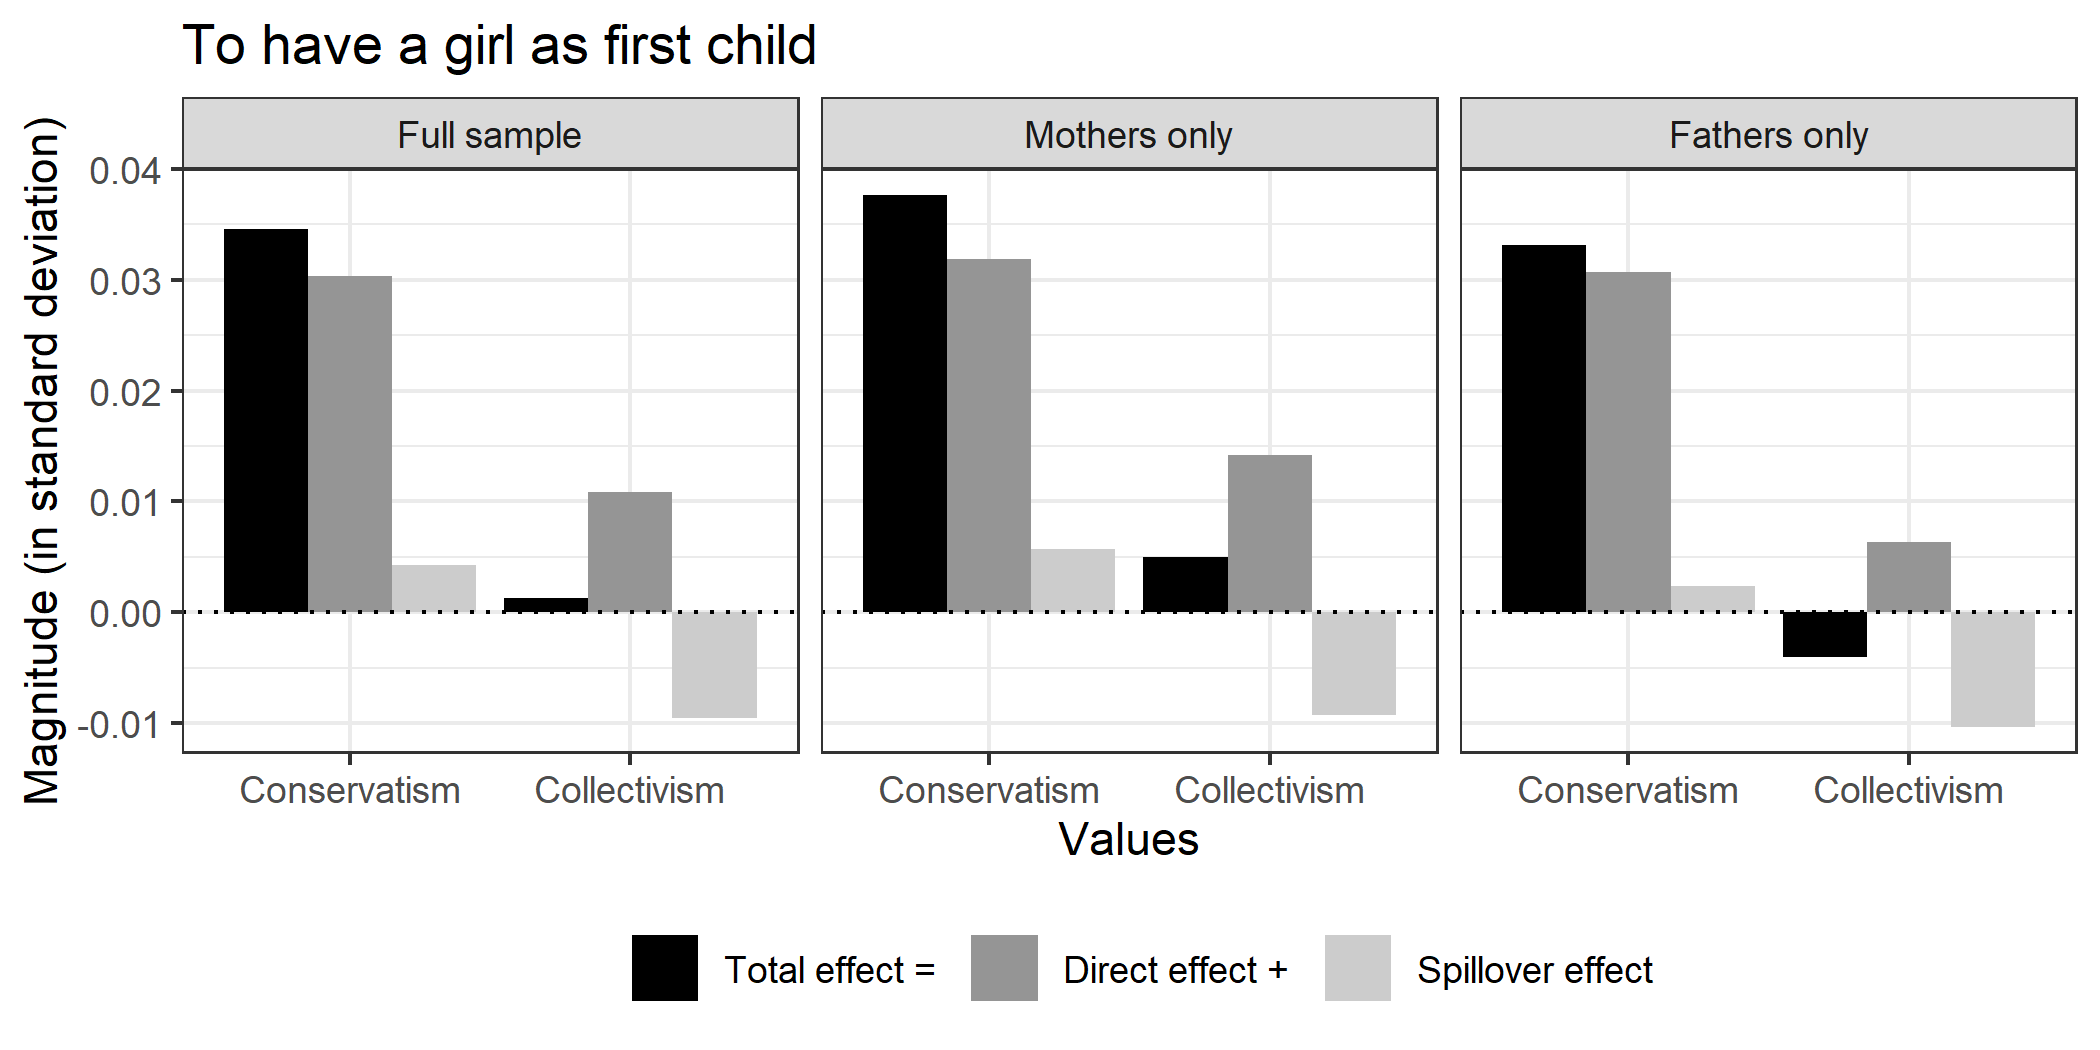
\includegraphics[width=\linewidth]{chap3/graphic/decomp-v5-GFGender.png}
    \hrulefill
	\vspace{-3em}
	\justify\singlespacing\footnotesize{\textit{Notes:} This figure presents the decomposition of the total effect of the girl-first life event on both values, Conservation and Collectivism, according to the parent. The magnitude of each effect is expressed in standard deviation.}
\end{figure}

\begin{figure}[!htb]
    \centering
    \caption{Decomposition of the effect of GirlFirst by education}
    \label{chap3-fig:sem-decomp-v5-GFEduc}
    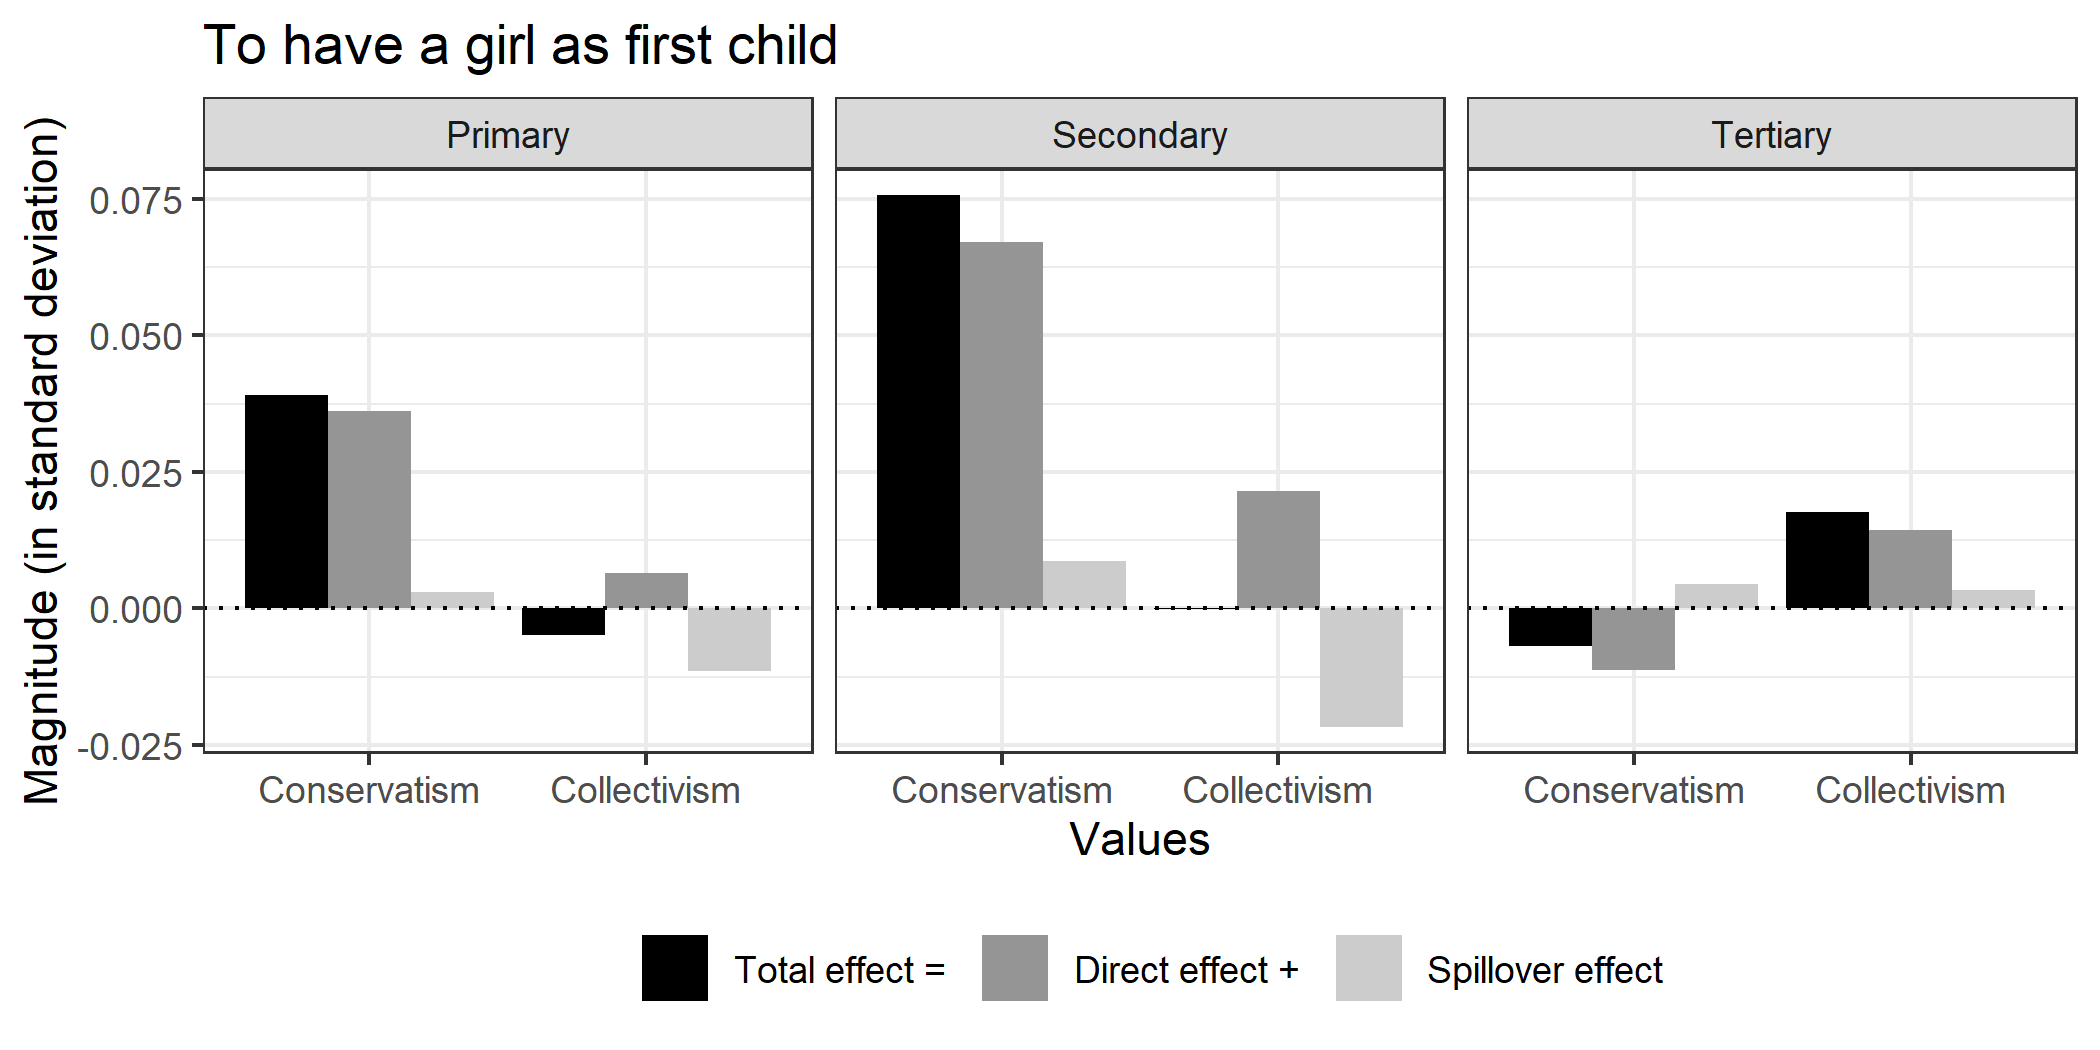
\includegraphics[width=\linewidth]{chap3/graphic/decomp-v5-GFEduc.png}
    \hrulefill
	\vspace{-3em}
	\justify\singlespacing\footnotesize{\textit{Notes:} This figure presents the decomposition of the total effect of the girl-first life event on both values, Conservation and Collectivism, according to education. The magnitude of each effect is expressed in standard deviation.}
\end{figure}

\begin{figure}[!htb]
    \centering
    \caption{Decomposition of the effect of GotCancer with and without the NCDS58 Age 50}
    \label{chap3-fig:sem-decomp-v5-GCNCDS58}
    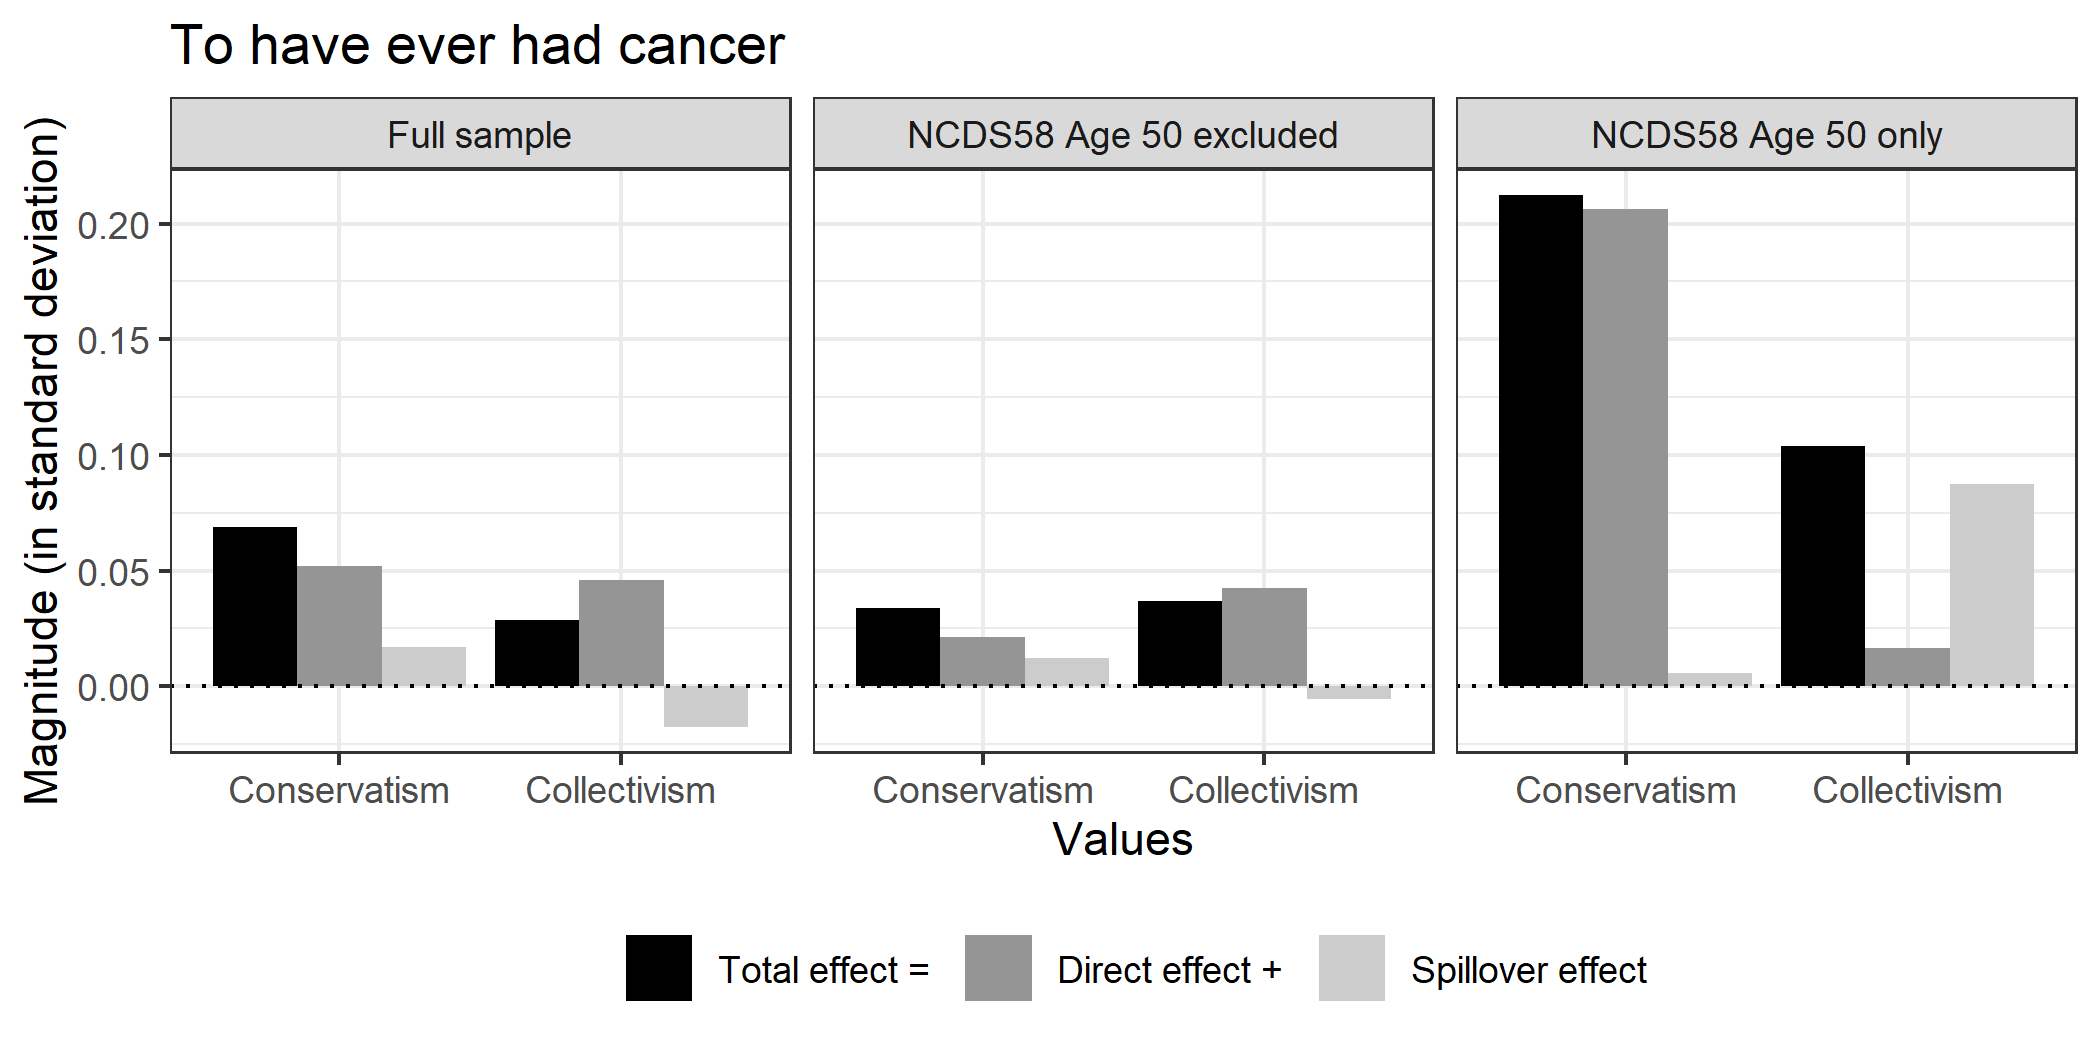
\includegraphics[width=\linewidth]{chap3/graphic/decomp-v5-GCNCDS58.png}
    \hrulefill
	\vspace{-3em}
	\justify\singlespacing\footnotesize{\textit{Notes:} This figure presents the decomposition of the total effect of the got-cancer life event on both values, Conservation and Collectivism, for the NCDS58 cohort at age 50 only and without them. The magnitude of each effect is expressed in standard deviation.}
\end{figure}

\begin{figure}[!htb]
    \centering
    \caption{Decomposition of the effect of GotCancer for those who never have had cancer before}
    \label{chap3-fig:sem-decomp-v5-GCNever}
    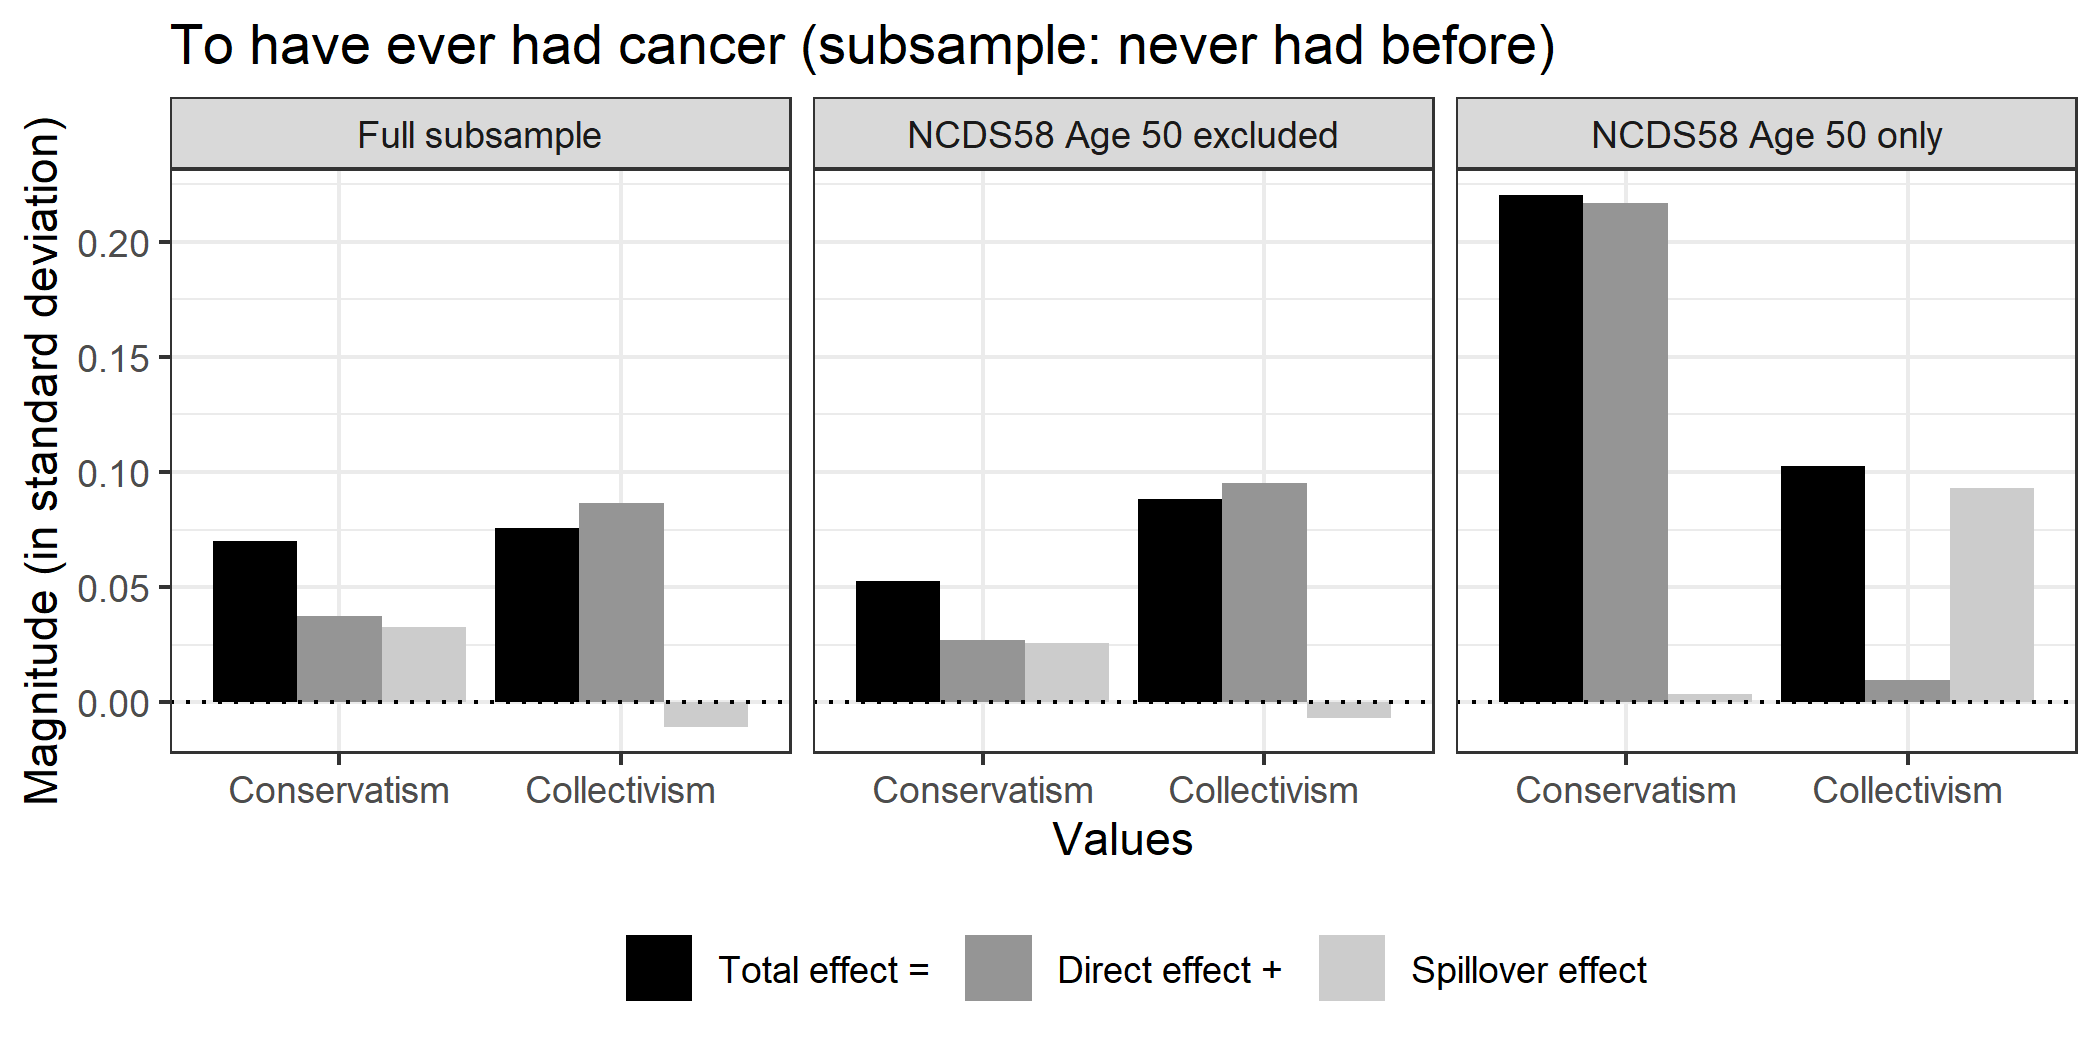
\includegraphics[width=\linewidth]{chap3/graphic/decomp-v5-GCNever.png}
    \hrulefill
	\vspace{-3em}
	\justify\singlespacing\footnotesize{\textit{Notes:} This figure presents the decomposition of the total effect of the got-cancer life event on both values, Conservation and Collectivism, for the NCDS58 cohort at age 50 only and without them. The magnitude of each effect is expressed in standard deviation.}
\end{figure}

\begin{figure}[!htb]
    \centering
    \caption{Decomposition of the effect of BeenUnemp by current activity status}
    \label{chap3-fig:sem-decomp-v5-BUActivity}
    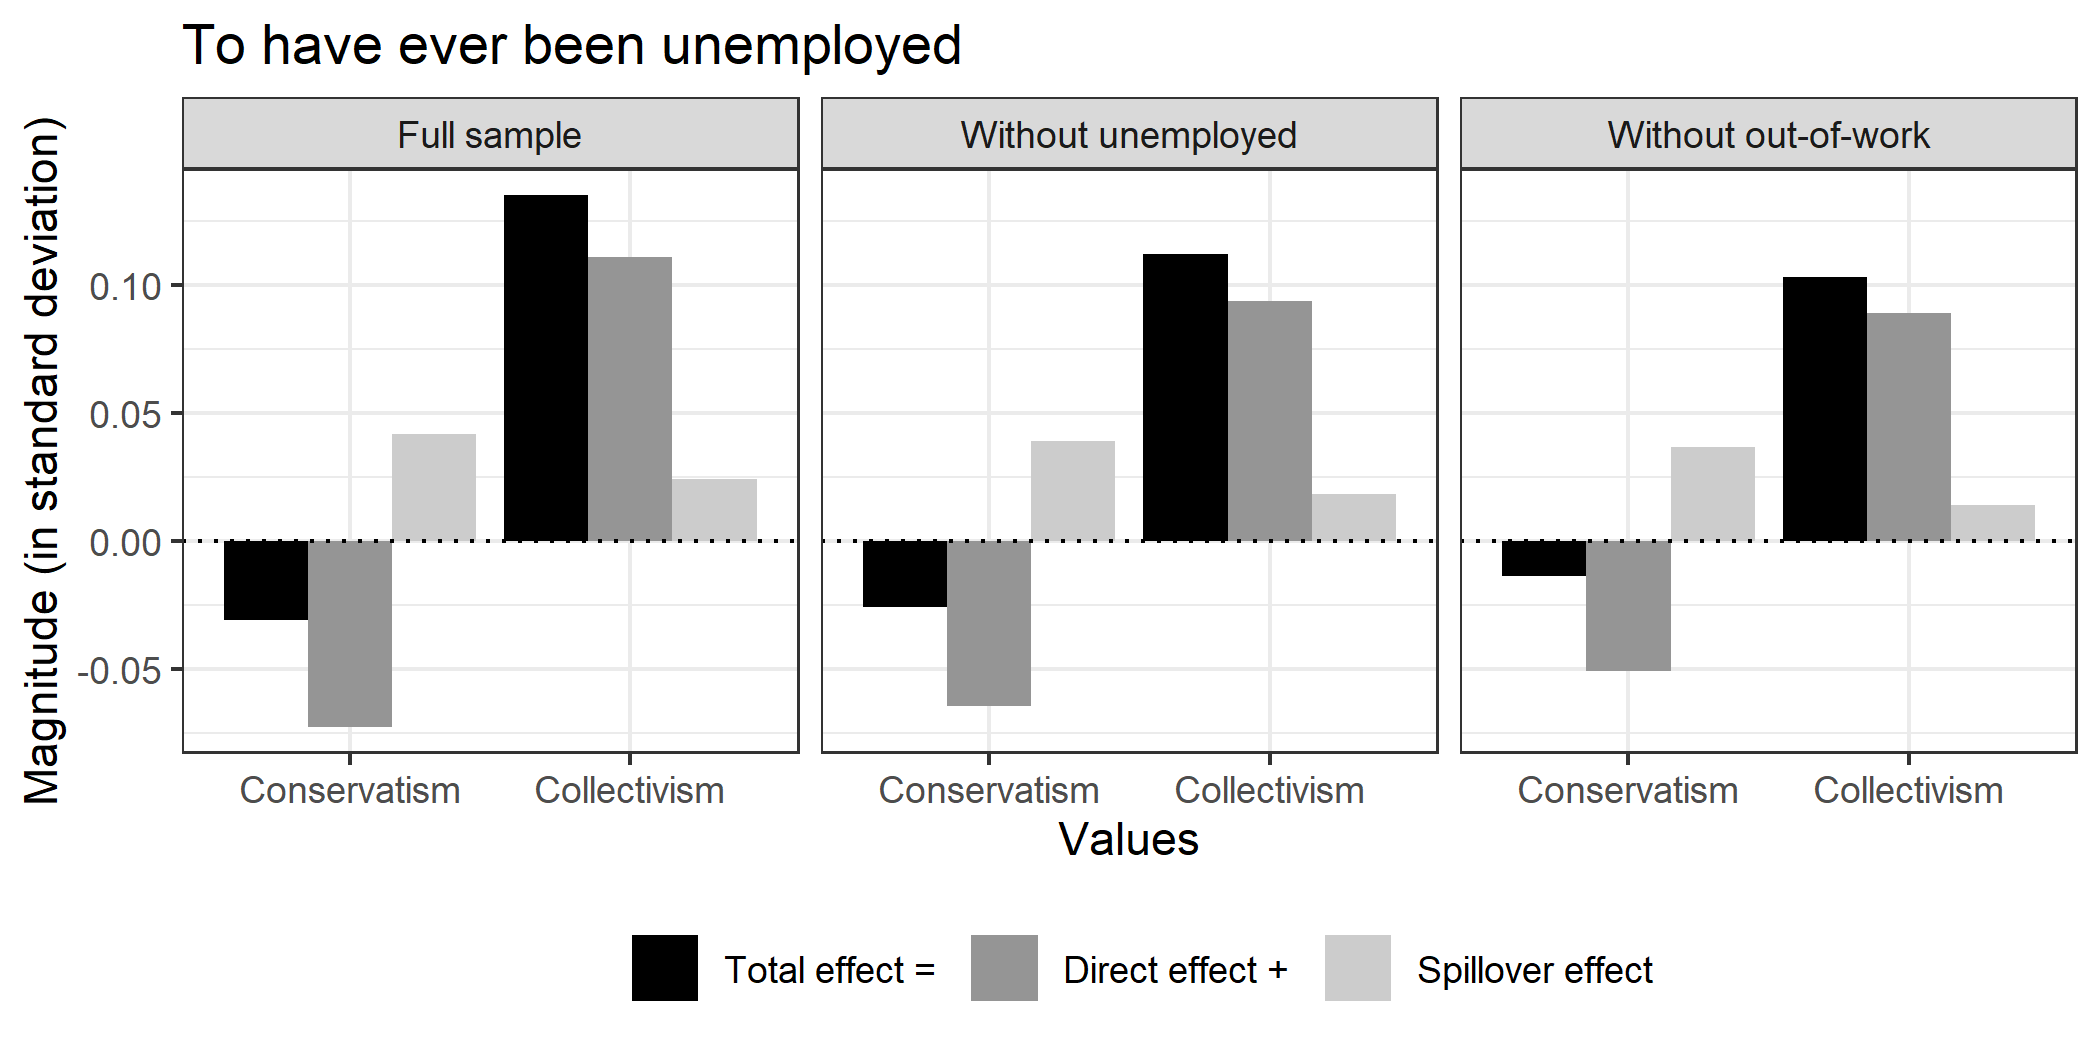
\includegraphics[width=\linewidth]{chap3/graphic/decomp-v5-BUActivity.png}
    \hrulefill
	\vspace{-3em}
	\justify\singlespacing\footnotesize{\textit{Notes:} This figure presents the decomposition of the total effect of the girl-first life event on both values, Conservation and Collectivism, according to the current activity status. The magnitude of each effect is expressed in standard deviation.}
\end{figure}